\documentclass[11pt]{article}
\usepackage[utf8]{inputenc}
\usepackage[T1]{fontenc}
\usepackage[margin=1in]{geometry}
\usepackage{mathtools,amsmath,amssymb,amsthm}
\usepackage{booktabs}
\usepackage{enumitem}
\usepackage{tikz}
\usetikzlibrary{arrows.meta,positioning}
\usepackage{url}
\usepackage[hidelinks]{hyperref}
\usepackage[capitalise]{cleveref}

\newtheorem{theorem}{Theorem}[section]
\newtheorem{lemma}[theorem]{Lemma}
\newtheorem{corollary}[theorem]{Corollary}
\newtheorem{proposition}[theorem]{Proposition}
\theoremstyle{definition}
\newtheorem{definition}[theorem]{Definition}
\newtheorem{example}[theorem]{Example}
\theoremstyle{remark}
\newtheorem{remark}[theorem]{Remark}

% Long Coq names cannot hyphenate; give the line breaker room.
\setlength{\emergencystretch}{3em}

% A gated Coq name, as it appears in coq/*.v; may break after an underscore.
\makeatletter\g@addto@macro{\UrlBreaks}{\do\_}\makeatother
\DeclareUrlCommand\coq{\urlstyle{tt}}
\newcommand{\gov}{\mathsf{gov}}
\newcommand{\reach}{\mathsf{reach}}
\newcommand{\valid}{\mathsf{valid}}

\title{Normalization confluence: an exact, mechanized theory of\\when repair can replace commutativity}
\author{Dayna Blackwell}
\date{Draft}

\begin{document}
\maketitle

\noindent\emph{Working draft. Sections are added as they are written; see docs/PAPER-OUTLINE.md.}

\setcounter{section}{2}
% Section 3. Drafted from docs/paper/section-3-skeleton.md. Every named result is a gated,
% axiom-free theorem in coq/*.v; statements are read from the source.

\section{The main result}\label{sec:main}

Replicas apply the same events in different orders, because networks delay, reorder and retry
messages, and every replica runs the same repair after each event to restore its invariants. The
question is when replicas that have seen the same events end in the same state. The answer has one
shape at every scale: raw states may differ along the way, and what has to agree is the result after
repair. This section states an exact condition at three scales, a single event
(\cref{sec:main-state}), finite histories (\cref{sec:main-history}) and infinite runs
(\cref{sec:main-recurrence}), together with the single-registry theorem that combines the first two
(\cref{sec:main-single}). The three conditions are not one equation. They form a proved hierarchy,
with counterexamples showing where each level stops (\cref{sec:main-hierarchy}).

Throughout, $X$ is a set of states and $N : X \to X$ is the repair. An event is a map
$e : X \to X$ on raw states; a replica applies an event and then repairs, so its step is
$x \mapsto N(e(x))$.

% ---------------------------------------------------------------------------------------------
\subsection{One event: state descent}\label{sec:main-state}

\begin{definition}[State descent; \coq{DescendsOn}]\label{def:descent}
An event $e$ \emph{descends} on a set $P \subseteq X$ when
\[
  N(e(N(x))) \;=\; N(e(x)) \qquad\text{for every } x \in P.
\]
\end{definition}

The condition says that applying the event to a state or to its repaired form gives the same result
after repair. Repairing early loses nothing the event can observe. For an idempotent repair the definition is the
standard compatibility of a map with the kernel of $N$ (\coq{descends_iff_respects}); what matters here is that
convergence forces it, at the states a system can reach.

\begin{example}[A shelf]\label{ex:shelf}
A shelf holds at most 5 items and has 4 in stock. The events are ``add 3'' and ``remove 1'', and the
repair caps the stock at 5, so $N(x) = \min(x, 5)$. Replica~A applies ``add 3'' (7), repairs (5), then
``remove 1'': it ends at 4. Replica~B applies ``remove 1'' (3), then ``add 3'' (6), and repairs: it
ends at 5. The two replicas saw the same events and ran the same repair, and they disagree.

State descent locates the failure. Take the raw state 7, just after ``add 3'', and let $e$ be
``remove 1''. Then $N(e(N(7))) = N(e(5)) = N(4) = 4$, while $N(e(7)) = N(6) = 5$. The event does not
descend at 7: removing an item before or after the cap is applied gives different answers.
\end{example}

In the single-registry setting of \cref{sec:main-single}, state descent is exactly one of the two
conditions convergence requires. There, the repair is built from a repair step $\rho$ that strictly
decreases a potential $\Phi : X \to \mathbb{N}$ on invalid states, and $N = \rho^{*}$ applies $\rho$
until the state is valid.

\begin{proposition}[\coq{state_descent_iff_cc2}]\label{prop:descent-cc2}
If $\Phi(\rho(s)) < \Phi(s)$ for every invalid $s$, then every event descends on all of $X$ under
$N = \rho^{*}$ if and only if
\[
  \rho^{*}(e(s)) \;=\; \rho^{*}(e(\rho(s))) \qquad\text{for every event } e \text{ and every invalid } s.
\]
\end{proposition}

The right-hand side is the condition called CC2 below: an event does not care whether one repair
step ran before it.

% ---------------------------------------------------------------------------------------------
\subsection{Finite histories: history descent}\label{sec:main-history}

A delivery model says which reorderings of a history count as the same delivery. Under free delivery
every permutation is allowed; under causal delivery, only orders consistent with a happens-before
relation; under at-least-once delivery, also duplicates; under declared independence, swaps of
declared pairs.

\begin{definition}[History descent]\label{def:history}
For a delivery model, given as an equivalence $\equiv$ on histories, and a start $s_0$, the system
satisfies \emph{history descent} when every two equivalent histories give the same result after
repair: $N(\mathrm{run}(h, s_0)) = N(\mathrm{run}(k, s_0))$ whenever $h \equiv k$, where
$\mathrm{run}$ applies the raw events in order.
\end{definition}

The raw runs in this definition never repair. A replica, however, repairs after every event. The next
lemma says that, given state descent, the two views agree, so a checker may work with repaired states
only.

\begin{lemma}[\coq{history_from_descent}]\label{lem:transfer}
Suppose every event descends on $X$. Write $\mathrm{grun}(h, x)$ for the run that applies the events
of $h$ to $x$ and repairs after each one. Then for every equivalence $\equiv$ on histories and every
start $s_0$,
\[
  \bigl(\forall h \equiv k.\; N(\mathrm{run}(h, s_0)) = N(\mathrm{run}(k, s_0))\bigr)
  \iff
  \bigl(\forall h \equiv k.\; \mathrm{grun}(h, N(s_0)) = \mathrm{grun}(k, N(s_0))\bigr).
\]
\end{lemma}

The proof is the observation that, under state descent, $N(\mathrm{run}(w, s_0)) =
\mathrm{grun}(w, N(s_0))$ for every word $w$ (\coq{normalization_descent}). Which reorderings preserve
the result depends on the delivery model; Section~5 gives one theorem pair that decides it for
each model above. Here only free delivery is needed, through the single-registry theorem.

% ---------------------------------------------------------------------------------------------
\subsection{The single-registry theorem}\label{sec:main-single}

A \emph{registry} fixes the states, a validity predicate $\valid$, the events, and the repair step
$\rho$ with its potential $\Phi$. Write $\gov(e) = \rho^{*} \circ e$ for the governed step. A
configuration is a pair $(\sigma, B)$ of a state and a buffer of pending events; a step either applies
a pending event to $\sigma$ or, when $\sigma$ is invalid, applies $\rho$. A normal form is a valid state
with an empty buffer. A state is \emph{reachable} from $s_0$, written $\reach(s_0, \sigma)$, when some
sequence of event and repair steps leads from $s_0$ to $\sigma$.

\begin{theorem}[Compensation commutativity; \coq{cc_exact}]\label{thm:cc}
Let $\Phi(\rho(s)) < \Phi(s)$ for every invalid $s$. For every start $s_0$, every configuration
$(\sigma, B)$ with $\reach(s_0, \sigma)$ has a unique normal form if and only if both of the following
hold at every state $\sigma$ reachable from $s_0$:
\begin{enumerate}[label=(CC\arabic*)]
  \item $\gov(e_2)(\gov(e_1)(\sigma)) = \gov(e_1)(\gov(e_2)(\sigma))$ for all events $e_1, e_2$;
  \item $\gov(e)(\sigma) = \gov(e)(\rho(\sigma))$ for every event $e$, when $\sigma$ is invalid.
\end{enumerate}
\end{theorem}

In words: replicas converge exactly when repaired events commute (CC1) and an event does not care
whether repair ran first (CC2), at the states they can reach. Termination of repair is the standing
hypothesis; it is the third condition of the theory, called WFC in the earlier papers.

The theorem reads directly in the vocabulary of the two descents. CC1 is history descent for free
delivery, stated on the governed steps, and CC2 is state descent on the reachable states.

\begin{corollary}[\coq{nd_derived_from}]\label{cor:descent-form}
Under the hypotheses of \cref{thm:cc}, every configuration $(s_0, B)$ has a unique normal form if and
only if the governed runs from $N(s_0)$ agree on every permutation of every history, and every event
descends on the states reachable from $s_0$.
\end{corollary}

Section~9 shows that this form is derived from the framework's kernels without using
\cref{thm:cc}.

\paragraph{Proof idea, and what is not new.}
Sufficiency is Newman's lemma restricted to the reachable states, with a case split on the two kinds
of critical peak: two events, and an event against a repair step. Necessity uses two small runs. The
buffer $[e_1, e_2]$ in both orders forces CC1; the buffer $[e]$ with the event first versus the repair
first forces CC2. Both ends of each run are normal forms, because $\rho^{*}$ always reaches a valid
state. The result is therefore the critical-pair theorem of Knuth and Bendix and of
Huet~\cite{huet1980}, specialized to a system whose critical pairs are already normal forms: that is
why ``joinable'' becomes ``equal'' and the converse costs nothing. The contribution is the condition
and its necessity at the reachable states, not the proof technique. Two counterexamples fix the
qualifiers: without the restriction to reachable states the converse fails
(\coq{rho_star_qualifier}, \coq{masked_cc1}).

% ---------------------------------------------------------------------------------------------
\subsection{Infinite runs: canonical recurrence}\label{sec:main-recurrence}

When repair may never stop, for example on networks of registries that feed each other around a
cycle, the question becomes one of long-run behavior. A system now has a finite set of actions $J$,
each with an update $u_j : X \to X$, and a schedule $\sigma : \mathbb{N} \to J$ picks the action at
each step. A schedule is \emph{fair} when every action is picked infinitely often, an action that
changes nothing at the current state being a no-op. At this scale $N$ may be any observation $N : X \to C$ of the state, for example its repaired
result. A run \emph{settles} on $c \in C$ when $N(x_n) = c$ for all large enough $n$.

A \emph{bad fair lasso} from $s_0$ for $c$ is a path from $s_0$ to a state $x$ followed by a
nonempty loop from $x$ back to $x$ that picks every action, with some state on the loop outside the
fiber $N^{-1}(c)$.

\begin{theorem}[Canonical recurrence; \coq{C1_closed}]\label{thm:c1}
Let $X$ be finite, and suppose the fiber $N^{-1}(c)$ is closed under every update. Then every fair run
from $s_0$ settles on $c$ if and only if there is no bad fair lasso from $s_0$ for $c$.
\end{theorem}

Settling fails exactly through a fair loop that leaves the target result. The kernel is the classical
fair-cycle characterization of Emerson and Lei~\cite{emersonlei1987}, read through $N$; its role here
is to classify how runs fail (oscillation, livelock, settling on the wrong state) in one vocabulary
(Section~6). Finiteness is needed for the exact form only: a bad fair lasso refutes settling
on any state space (\coq{C1_refutes}).

At this scale the condition reads repair only through its result.

\begin{proposition}[\coq{canon_settles_quotient_invariant}]\label{prop:quotient}
Suppose the updates $u_j$ respect $N$, that is $N(x) = N(y)$ implies $N(u_j(x)) = N(u_j(y))$, and
let $u'_j$ satisfy $N(u'_j(x)) = N(u_j(x))$ for every action and state. If $N(s'_0) = N(s_0)$, then
every fair run of $u$ from $s_0$ settles on $c$ if and only if every fair run of $u'$ from $s'_0$
does.
\end{proposition}

% ---------------------------------------------------------------------------------------------
\subsection{How the conditions relate}\label{sec:main-hierarchy}

The three conditions are not one equation. State descent and history descent are independent of each
other; together, with terminating repair, they are exactly convergence of a single registry
(\cref{cor:descent-form}); and terminating repair connects them to settlement through Newman's lemma
(Section~8). Each separation is witnessed by a mechanized counterexample.

\begin{proposition}\label{prop:separations}
\leavevmode
\begin{enumerate}[label=(\alph*)]
  \item \emph{State descent without history descent} (\coq{descent_not_history}). With $N$ the
    identity every event descends, and two events that do not commute give different results for the
    two orders of one history.
  \item \emph{History descent without state descent} (\coq{history_not_descent}). With one event,
    the successor map on $\mathbb{N}$, and the repair $N$ that sends $0$ and $1$ to $0$ and fixes every
    other number, every reordering of a history is the history itself, so history descent holds; but
    $N(e(N(1))) = N(1) = 0$ while $N(e(1)) = N(2) = 2$.
  \item \emph{Infinite runs need descent} (\coq{trajectory_needs_descent}). There are two systems whose
    updates have the same image under $N$ at every state, neither of which respects $N$, such that,
    from the same start, every fair run of one settles on \textsf{true} and every fair run of the
    other settles on \textsf{false}.
\end{enumerate}
\end{proposition}

\begin{figure}[t]
\centering
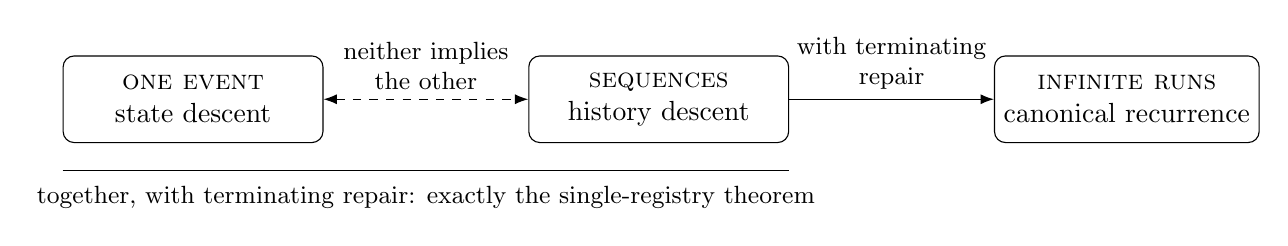
\begin{tikzpicture}[
  box/.style={draw, rounded corners, minimum width=3.3cm, minimum height=1.1cm, align=center},
  lab/.style={font=\small, align=center}]
  \node[box] (s) {\textsc{one event}\\ state descent};
  \node[box, right=2.6cm of s] (h) {\textsc{sequences}\\ history descent};
  \node[box, right=2.6cm of h] (c) {\textsc{infinite runs}\\ canonical recurrence};
  \draw[{Latex}-{Latex}, dashed] (s) -- node[lab, above] {neither implies\\ the other} (h);
  \draw[-{Latex}] (h) -- node[lab, above] {with terminating\\ repair} (c);
  \draw ([yshift=-0.35cm]s.south west) -- ([yshift=-0.35cm]h.south east)
    node[lab, midway, below=2pt] {together, with terminating repair: exactly the single-registry theorem};
\end{tikzpicture}
\caption{The three conditions and the proved relations between them
(\cref{prop:separations,cor:descent-form,thm:c1}).}
\label{fig:hierarchy}
\end{figure}

Every condition in this section is exact: necessary and sufficient, with each hypothesis shown to be
needed by a counterexample. Section~4 reads the single-registry theorem against CRDTs, the case
where repair never runs, and Sections~5 to~8 give the
three-layer framework that organizes these conditions across the regimes of the map.


\begin{thebibliography}{9}
\bibitem{huet1980} G.~Huet. Confluent reductions: abstract properties and applications to term
  rewriting systems. \emph{Journal of the ACM} 27(4):797--821, 1980.
\bibitem{emersonlei1987} E.~A.~Emerson and C.-L.~Lei. Modalities for model checking: branching time
  logic strikes back. \emph{Science of Computer Programming} 8(3):275--306, 1987.
\end{thebibliography}

% Section 4. Drafted from docs/PAPER-OUTLINE.md section 4 and docs/SUBSUMPTION.md. Every named
% result is a gated, axiom-free theorem in coq/*.v; statements are read from the source.

\section{CRDTs, invariant confluence, and what repair adds}\label{sec:crdt}

Two bodies of work answer neighboring questions. Conflict-free replicated data types (CRDTs)
obtain convergence by designing operations so that order never matters~\cite{shapiro2011}.
Invariant confluence asks which transactions can run without coordination while preserving an
invariant~\cite{bailis2014}. This section places normalization confluence against both, precisely:
CRDTs are the case where repair does nothing (\cref{sec:crdt-identity}); repair enlarges which
operations can be used, but not which behaviors converge (\cref{sec:crdt-readings}); and invariant
confluence is a different question, because there the invariant is checked and never repaired
(\cref{sec:crdt-iconf}).

% ---------------------------------------------------------------------------------------------
\subsection{CRDTs are the case where repair does nothing}\label{sec:crdt-identity}

In the terms of \cref{sec:main}, a CRDT is a system whose repair $N$ is the identity. State descent,
$N(e(N(x))) = N(e(x))$, then holds for every event, so convergence comes down to history descent
alone: every reordering the delivery model allows must give the same state. The classical CRDT
conditions are what this reduces to under the two delivery models CRDTs are built for. Write
$\mathrm{gstep}(e) = N \circ e$ for the governed step.

\begin{theorem}[The compensation-free boundary; \coq{crdt_boundary} (a), (b), (b')]\label{thm:boundary}
Let $N$ be the identity.
\begin{enumerate}[label=(\alph*)]
  \item \emph{Causal exactly-once delivery.} For every irreflexive happens-before relation, the
    governed steps converge causally from every start (any two causally consistent orders of the
    same events reach the same state) if and only if concurrent raw operations commute at every
    state.
  \item \emph{Unordered at-least-once delivery.} For every event range $R$ with decidable equality
    and every start $s_0$, any two deliveries over $R$ with the same set of events, in any order and
    with any duplication, reach the same state from $s_0$ if and only if the raw operations are
    commutative and idempotent at every state reachable from $s_0$.
  \item[(b$'$)] \emph{The semilattice form.} If moreover $R$ is finite and state equality is
    decidable, the convergence of (b) holds if and only if the raw operations have a
    join-semilattice representation on the states reachable from $s_0$: some join is a semilattice
    there and every event acts as $e(s) = s \sqcup e(s_0)$.
\end{enumerate}
\end{theorem}

Part (a) is the op-based (CmRDT) condition and part (b$'$) the state-based (CvRDT) condition of
Shapiro et al.~\cite{shapiro2011}, each in exact form: Shapiro et al.\ give them as sufficient
conditions, and the theorem shows they are also necessary, on the states a system can reach. The
qualifiers are needed: reachability cannot be dropped (\coq{clamp_reach_qualifier}), a semilattice on
all of the state space is too strong (\coq{naive_cvrdt_iff_fails}), and both commutativity and
idempotence are needed in (b) (\coq{lww_not_conv}, \coq{add_cc_not_alo}). The exact conditions behind
(a) and (b) are \coq{causal_convergence_exact} and \coq{merge_action_exact}; the theorem instantiates
them at the identity repair.

% ---------------------------------------------------------------------------------------------
\subsection{Two readings of ``repair enlarges what converges''}\label{sec:crdt-readings}

The usual claim for a repair-based design is that it reaches systems CRDTs cannot. The claim is true
in one reading and false in another, and the paper separates them.

\paragraph{Operations: strict.}
Some raw operations converge only with repair.

\begin{proposition}[\coq{crdt_boundary} (c)]\label{prop:witness}
Take a single Boolean whose only valid value is \textsf{false}, two events with raw transitions
$\mathsf{settrue}(s) = \textsf{true}$ and $\mathsf{flip}(s) = \neg s$, and the repair that resets to
\textsf{false}. The governed system converges under causal exactly-once delivery from every start
and under unordered at-least-once delivery from every start. The raw operations satisfy none of the
conditions of \cref{thm:boundary}: they do not commute where the two events are concurrent, the
system built from them without repair fails to converge under both delivery models, they are neither
commutative nor idempotent at a reachable state from any start, and they have no semilattice
representation on the reachable states.
\end{proposition}

So no system without repair that uses these raw transitions converges, while the repaired system
does. The separation is sharpened in \coq{witness_ops_not_commute}, \coq{witness_raw_not_causal},
\coq{witness_not_cvrdt_order} (no partial order on the Booleans makes both raw operations
inflationary) and \coq{witness_not_cvrdt_exact}.

\paragraph{Behavior: not strict.}
The exact conditions behind \cref{thm:boundary} hold for any step function, not only for raw
operations. Read at the governed step $\mathrm{gstep}(e) = N \circ e$, they say:

\begin{corollary}[\coq{causal_convergence_exact}, \coq{merge_action_exact}, at the governed step]\label{cor:behavior}
For any repair $N$:
\begin{enumerate}[label=(\alph*)]
  \item for an irreflexive happens-before relation, the governed system converges causally from
    every start if and only if governed steps of concurrent events commute at every state;
  \item from a start $s_0$, the governed system converges under unordered at-least-once delivery if
    and only if the governed steps are commutative and idempotent at every state reachable from
    $s_0$.
\end{enumerate}
\end{corollary}

These are the CmRDT and the commutative-idempotent conditions, stated for the governed steps. So
every convergent governed system is a CRDT on its own governed steps, at the states it reaches. The
witness of \cref{prop:witness} is an instance: its governed behavior is the constant
\textsf{false}, and its governed steps are a CvRDT with join $\wedge$
(\coq{witness_governed_constant}).

\paragraph{What repair adds.}
Normalization confluence does not reach convergent behaviors that CRDTs cannot. What it adds is a
way to build them. A designer writes the operations the application needs, which need not commute,
and a repair that restores the invariants; the exact conditions of \cref{sec:main}, state descent
and history descent, decide whether the combination converges, which is to say whether its governed
steps form a CRDT. The design freedom is in the operations, and the guarantee is checked rather than
designed in. \cref{sec:gsm} describes a checker that runs these conditions at build time.

% ---------------------------------------------------------------------------------------------
\subsection{Invariant confluence: checked, not repaired}\label{sec:crdt-iconf}

Invariant confluence~\cite{bailis2014} asks whether a set of transactions can run on replicas that
merge their states without coordination and still preserve an invariant $I$. A transaction commits
only if its local result satisfies $I$, and a merge can never be refused. The invariant is checked,
never repaired. This is a different question from the one normalization confluence answers, and the
two meet in one place: the merge.

Model the invariant as the solution set of a constraint problem and the merge as an operation
applied item by item. In the constraint-satisfaction terms of \cref{sec:layer-b}, the merge is then
a binary operation on states, and invariant confluence becomes a statement about it.

\begin{theorem}[\coq{pol_iconfluent}, \coq{iconf_iff_pol_reach}]\label{thm:iconf}
\leavevmode
\begin{enumerate}[label=(\alph*)]
  \item If the item-wise merge is a polymorphism of the invariant's constraint language, every set of
    transactions is invariant confluent.
  \item Exactly: when $I$ holds at the start and reads finitely many items, a set of transactions is
    invariant confluent if and only if the merge is a polymorphism of the relation of states
    reachable under those transactions with $I$ preserved.
\end{enumerate}
\end{theorem}

The restriction to reachable states is necessary, as Whittaker and
Hellerstein~\cite{whittaker2018} observed. A mechanized counterexample makes it concrete
(\coq{uq_not_pol}): with two versions $a$ and $b$, merge by set union, the invariant ``not both
present'' and the single transaction ``add $a$'', the transactions are invariant confluent, but
union does not preserve the invariant on all states. Bailis et al.'s main theorem, that a
coordination-free, available, convergent and invariant-preserving execution exists exactly for
invariant-confluent transactions, holds in a replica model mechanized in the same file
(\coq{replica_exact}); necessity for arbitrary protocols would need a model of partitions that the
development does not have.

Repair changes the picture. With the same invariant and both transactions ``add $a$'' and ``add
$b$'', the transactions are not invariant confluent. With the repair
$N(x, y) = (x,\, y \wedge \neg x)$, which drops $b$ whenever $a$ is present, state descent and
history descent both hold, every repaired state satisfies the invariant, and replicas that exchange
repaired states agree with the repaired run of the joint history (\coq{repair_enlarges}). The caveat
is that this repair can undo a committed write, which Bailis et al.'s model forbids; the comparison is
between two models, not a strengthening of theirs.


% Section 5. Drafted from docs/PAPER-OUTLINE.md section 5 and docs/THEORY.md "Layer A". Every named
% result is a gated, axiom-free theorem in coq/*.v (PresentedExecution.v unless noted).

\section{Layer A: execution}\label{sec:layer-a}

Layer~A asks which executions count as the same. Every delivery model in the regime map answers that
question differently: free delivery allows every reordering, causal delivery only those consistent
with happens-before, at-least-once delivery also identifies a duplicate with its first landing, and a
live reconfiguration identifies an event before the switch with its translation after it. This section
states the question once, in a form every model fits, and proves the two principles that answer it.
The exact history results of the map are then instances, recovered with their original statements.

% ---------------------------------------------------------------------------------------------
\subsection{Presented executions}

Executions are words over a set of labels $L$, but not every word is an execution: causal
consistency, typed phases and legal duplicate landings rule some out. The data of a delivery model is
therefore a \emph{presented admissible path system}:
\begin{itemize}[nosep]
  \item a predicate $\mathrm{Adm}$ on words, the admissible executions, closed under prefixes where a
    theorem needs it ($\mathrm{AdmPrefix}$);
  \item generator pairs $\mathrm{Gen}(p, u, v)$: at the point $p$, the fragments $u$ and $v$ are
    interchangeable, for example a swap of independent events $[a; b] \sim [b; a]$, a legal duplicate
    landing $[a; a] \sim [a]$, or a switch square between typed phases;
  \item the generated equivalence $\mathrm{PEq}$: the equivalence closure, through admissible words
    only, of the whiskered pairs $p \cdot u \cdot w \sim p \cdot v \cdot w$.
\end{itemize}
Free delivery is the degenerate case: with every word admissible and generators independent of the
point, $\mathrm{PEq}$ is the monoid congruence the pairs generate (\coq{free_congruence}), and for
adjacent swaps it is equality up to permutation (\coq{swap_peq_perm}). This is the quotient a string
presentation defines, as in trace theory~\cite{cartier1969,mazurkiewicz1977}.

A semantics $\mathrm{sem}$ on words is compared by an equivalence $\approx$; for a state machine,
$\mathrm{sem}(t)$ is the repaired state after running $t$ from the start. \emph{Invariance}
($\mathrm{PInv}$) says that $\mathrm{sem}$ is constant up to $\approx$ on each $\mathrm{PEq}$ class.
This is history descent (\cref{def:history}) for the delivery model the presentation describes.

% ---------------------------------------------------------------------------------------------
\subsection{The two principles}

The \emph{continuation closure} $\mathrm{PPC}$ is the least relation that contains every seed
$(p \cdot u,\, p \cdot v)$ with both sides admissible and is closed under appending the same event to
both sides while both stay admissible. Under prefix closure it is exactly the set of admissible
whiskered pairs (\coq{ppc_iff_whisk}).

\begin{theorem}[The closure principle; \coq{closure_exact}]\label{thm:p2}
If $\mathrm{Adm}$ is closed under prefixes, then invariance holds if and only if $\mathrm{sem}$ agrees,
up to $\approx$, on every pair in the continuation closure.
\end{theorem}

Invariance always implies agreement on the seeds themselves (\coq{seeds_necessary}), but the seeds
alone are not enough. A hidden register makes the gap concrete (\coq{hw_seeds_insufficient}): events
write a register the observation does not show, and a later event reveals it. Every swap seed is then
observationally equal at its point, yet invariance fails; the separating pair is a seed continued by
the reveal (\coq{hw_closure_witness}). The next principle says when the seeds do suffice.

\begin{theorem}[The local principle; \coq{local_exact}]\label{thm:p1}
Let $Q$ be a predicate on words that holds on both sides of every seed and is kept by admissible
extension, and suppose the semantics respects the future on $Q$: whenever $t$ and $t'$ satisfy $Q$,
$t \cdot e$ and $t' \cdot e$ are admissible, and $\mathrm{sem}(t) \approx \mathrm{sem}(t')$, then
$\mathrm{sem}(t \cdot e) \approx \mathrm{sem}(t' \cdot e)$. If $\mathrm{Adm}$ is closed under
prefixes, invariance holds if and only if every generator pair is observationally equal at its
point: $\mathrm{sem}(p \cdot u) \approx \mathrm{sem}(p \cdot v)$ whenever $\mathrm{Gen}(p, u, v)$ and both
sides are admissible.
\end{theorem}

With $Q$ true everywhere this is \coq{local_exact_all}, and the future-respecting hypothesis follows
when the observation is compatible with the steps (\coq{resp_of_compat}). In the hidden register it is
exactly that hypothesis that fails (\coq{hw_not_resp}). Both principles are elementary facts about
congruences generated by local pairs, in the style of semigroup presentations~\cite{howie1995}; the
work is in fitting every delivery model to them.

State descent is not a generator. It runs one word from two states, $s$ and $N(s)$, so it is a
relation on states, not a pair of parallel paths from one point. It enters through the semantics:
under state descent the repaired raw semantics and the governed semantics from $N(s_0)$ are the same
function on words, so they pose the same invariance question for every presentation
(\coq{state_side_transfer}; \cref{lem:transfer} is the special case of equality on histories).
Paths quotient histories; states quotient by repair.

% ---------------------------------------------------------------------------------------------
\subsection{The history results as instances}

Each exact history result of the map is recovered from the local or the closure principle with its original statement, over the
original module's own predicates (\cref{tab:layer-a}).

\begin{table}[t]
\centering\footnotesize
\setlength{\tabcolsep}{4pt}
\begin{tabular}{@{}p{2.4cm}p{4.0cm}p{1.9cm}p{6.0cm}@{}}
\toprule
Delivery model & Recovered as & Principle & Admissible words; generators \\
\midrule
Causal delivery & \coq{PresentedExecution.causal_exact_recovered} & local & causally consistent words; adjacent swaps of concurrent events at a causal point \\
Declared independence & \coq{tconv_exact_recovered} & local & causal histories; swaps of declared pairs (the trace monoid) \\
At-least-once & \coq{causal_alo_idem_recovered}, \coq{alo_exact_recovered} & local & at-least-once deliveries, causal (first name) or in any order (second); concurrent swaps and the landing $[a; a] \sim [a]$ after a first delivery \\
Live switch & \coq{det_live_recovered} & local, $Q$ = past the switch & typed phases; switch squares and post-switch swaps \\
Barrier, modulo a migration & \coq{amodm_closure_recovered} & closure & every word; adjacent swaps (the migration is not compatible with the steps) \\
\bottomrule
\end{tabular}
\caption{Exact history results recovered from the two principles. Each recovered theorem states the
original's conclusion over the original's predicates; the proofs go through \cref{thm:p1,thm:p2}.}
\label{tab:layer-a}
\end{table}

Three of these are not trace monoids. At-least-once delivery identifies a word with a shorter one,
the live switch has typed phases with labels that change at the switch, and the barrier case needs the closure principle
because the migration does not respect the future of the old configuration's steps. The live switch
is the instance where $Q$ matters: the migration does not respect the old configuration's future, but
every seed ends past the switch, where the new configuration's steps respect its observation.

\paragraph{The cost of fitting a model.}
The generic theorems are short; fitting a delivery model to them is not. Each recovery has to show
that the model's notion of ``same delivery'' is exactly the generated equivalence of its presentation,
an adequacy argument about words that does not involve the semantics. For at-least-once delivery that
argument is about 250 lines of word combinatorics. The recoveries therefore compress the history
results into one theorem pair plus a per-model adequacy cost, and the cost is part of the claim.

\paragraph{Not an instance.}
The single-registry theorem's commutation condition CC1 is not a row of this table. Its ambiguity is a
peak of a rewrite system in which repair steps interleave with events, not a pair of event words.
\cref{sec:base-case} combines the local principle on free delivery with a classification of those peaks to derive it.

% Section 6. Drafted from docs/PAPER-OUTLINE.md section 6 and docs/THEORY.md "Layer C". Every named
% result is a gated, axiom-free theorem in coq/*.v (CanonicalRecurrence.v unless noted).

\section{Layer C: long-run behavior}\label{sec:layer-c}

Layer~C asks whether runs reach a consistent state and which one. It is the scale of
\cref{sec:main-recurrence}, where repair may never stop: networks of registries that feed each other
around a cycle, resolvers that iterate to a fixed point, schedules that interleave updates
indefinitely. This section states one kernel for that scale, recovers the settlement results of the
map through it, and classifies every way a run was found to fail in one vocabulary.

% ---------------------------------------------------------------------------------------------
\subsection{The kernel}

A system has states $X$ with decidable equality, a list of actions $J$, and an update $u_j : X \to X$
for each action, applied asynchronously: a schedule picks one action per step, and it is fair when
every action is picked infinitely often. A \emph{fair lasso} from $s_0$ is a word $p$ that reaches a
state $x$, followed by a nonempty word $q$ that returns $x$ to itself and picks every action; its loop
states are the states $q$ visits. Let $N : X \to C$ be an observation and $c$ a target.

\begin{theorem}[C1; \coq{C1_closed}, \coq{C1_nn}]\label{thm:c1-kernel}
On a finite $X$, every fair run from $s_0$ is eventually always in $N^{-1}(c)$ if and only if no fair
lasso from $s_0$ has a loop state outside $N^{-1}(c)$. The equivalence is constructive when the fiber
is closed under every update (\cref{thm:c1}), and holds for every fiber in double-negated form.
\end{theorem}

\begin{theorem}[C2; \coq{C2}, \coq{C2_loops}]\label{thm:c2}
On a finite $X$, every fair run from $s_0$ eventually stays at a state fixed by every update if and
only if every fair lasso from $s_0$ has a single loop state, and that state is fixed by every update.
\end{theorem}

C1 asks whether runs settle on the right result; C2 asks whether they settle at all. The refutation
direction needs no finiteness: a bad fair lasso refutes settling on any state space
(\coq{C1_refutes}, \coq{bad_lasso_refutes}). This is the classical characterization of fair
behavior by reachable accepting cycles~\cite{clarke1986,emersonlei1987,vardi1986}, and it is not
claimed as new. The question this section answers is whether it compresses the development's
settlement results.

% ---------------------------------------------------------------------------------------------
\subsection{The settlement results as short bridges}

Each settlement result of the map was recovered by proving that no bad fair lasso exists and reading
settlement off C1 or C2. The argument for each is between 5 and 11 lines, over a shared,
regime-independent toolkit: pigeonhole on finite runs, inflationary loops, and a floor lemma for
loops below a fixed point.

\begin{itemize}[nosep]
  \item \emph{Chaotic iteration reaches the least fixed point} (\coq{chaotic_reaches_lfp_lasso}): a fair
    loop at a reachable state is inflationary, so it is a single fixed point, which is the least one.
  \item \emph{Signed networks settle} (\coq{signed_settlement_lasso}): the run from the bottom under the
    loop's word stabilizes at a fixed point below the loop, so from sound starts every fair loop is a
    single fixed point.
  \item \emph{and settle on the right fixed point} (\coq{signed_fidelity_lasso}): the run from the top
    bounds every loop by a fixed point, which is unique, so every recurrent class is that fixed point.
  \item \emph{Fair flush} (\coq{fairflush_lasso}, \coq{fairflushR_lasso}): the originals are C2.
\end{itemize}

A cycle that is not fair does not refute anything. The development has a bad cycle that never picks
one of the actions, in a network where every fair run settles
(\coq{nonfair_cycle_not_refuting}).

% ---------------------------------------------------------------------------------------------
\subsection{How runs fail}

Every long-run obstruction found in the map is a fair lasso, and C1 and C2 tell the kinds apart
(\coq{lasso_classification}).

\begin{itemize}[nosep]
  \item \emph{Oscillation.} A negation cycle is a bad fair lasso with more than one loop state; it is
    bad for every target.
  \item \emph{Livelock.} A bad fair lasso exists although the repair has exactly one fixed point
    (\coq{flip2_fair_lasso}); this is the B to C interface's counterexample of \cref{sec:interfaces}.
  \item \emph{Settling on the wrong state.} A single settled loop state in the wrong fiber: C2 holds and
    C1 fails (\coq{copyback_ghost_lasso}).
  \item \emph{Several fixed points.} Several reachable single-state loops: C2 holds and every target
    fails C1.
  \item \emph{Semantic oscillation.} A fair raw oscillation $a \to b \to a$ with $N(a) = N(b)$: C2 fails
    and C1 holds (\coq{semantic_oscillation}). The run never stops moving, but its repaired result
    never changes.
\end{itemize}

\noindent
A good monotone resolver has no bad fair lasso from any start. The last kind is why C1 and C2 are
separate conditions: a system can converge in the sense that matters, its result after repair, while
never quiescing.

% ---------------------------------------------------------------------------------------------
\subsection{Boundaries}

The recoveries are of finite fragments. Every bridge assumes a finite, listed state type, while the
originals assume only finite height, which allows infinitely many states; the chaotic-iteration bridge
also needs a finite list of components. The strong form of C1 is classical in general: on a four-state
instance with no bad fair lasso, strong settlement implies the limited principle of omniscience
(\coq{lpo_leak}). The recoveries avoid this because their targets are fixed points, whose fibers are
closed under the steps. Extending the kernel to finite-height state spaces with infinitely many states
is open.

% Section 7. Drafted from docs/PAPER-OUTLINE.md section 7 and docs/THEORY.md "Layer B". Every named
% result is a gated, axiom-free theorem in coq/*.v (TransportCSP.v and TransportCSPHard.v unless noted).

\section{Layer B: consistent states}\label{sec:layer-b}

Layer~B asks which states are consistent. It is a static question about a network's equations, not
about any run: when registries pass values along transport maps, a consistent assignment is one that
every map respects. This section shows that the question is a finite-domain constraint satisfaction
problem, that the fixed points of the repair dynamics are exactly its solutions, and that the
development's results sit at known points of the algebraic classification of such problems. Little of
the mathematics here is new; the section's role is to place consistency where a mature theory applies,
and to connect it to settlement through the interface of \cref{sec:interfaces}.

% ---------------------------------------------------------------------------------------------
\subsection{Consistency as constraint satisfaction}

Fix a finite family $F$ of transport maps on a finite set $D$. The \emph{template} $\Gamma_F$ consists
of the graphs $\{(x, f(x))\}$ of the maps in $F$, together with the unary relations $\{c\}$ for values
that some vertices are pinned to. A network whose edges are labeled by maps in $F$, with some vertices
pinned, is then an instance of $\mathrm{CSP}(\Gamma_F)$.

\begin{theorem}[\coq{section_iff_csp}, \coq{edge_fixed_iff_csp}]\label{thm:csp}
An assignment of values to the vertices of such a network is a section, a consistent assignment that
every edge's map respects, if and only if it is a solution of the corresponding instance of
$\mathrm{CSP}(\Gamma_F)$. Moreover, for a network without pinned vertices on a store with the usual
read and write laws, the states fixed by every edge repair of the network's dynamics are exactly those
solutions.
\end{theorem}

\emph{Proof idea.} The correspondence is unfolding: the constraint of an edge $u \to v$ labeled $f$ holds
at an assignment $s$ exactly when $f(s_u) = s_v$ (\coq{csat_econ}), and a pin constraint exactly when
the pinned value is taken (\coq{csat_pcon}), so sections agreeing with the pins are the solutions
(\coq{section_solution}); each constraint uses the graph of its edge's label or a pin, so the instance
is over $\Gamma_F$. Finiteness of $F$ and $D$ is not used. For the dynamics, the repair
$s[v := f(s_u)]$ fixes $s$ exactly when $f(s_u) = s_v$: reading $v$ after the write gives one
direction, and writing back the value just read leaves the store unchanged for the other
(\coq{erep_fixed_iff}). Taking every edge gives \coq{edge_fixed_iff_section}, and the correspondence turns
sections into solutions.

Merges in which a vertex reads several inputs are graphs of $k$-ary maps and fit the same way
(\coq{hsection_iff_csp}). The identification of global sections with constraint solutions is known in
general, from the sheaf-theoretic treatment of contextuality~\cite{abramsky2011,abramsky2014}; what is proved here
is its form for transport networks, together with the link to the dynamics.

An operation is a \emph{polymorphism} of the graph of $f$ exactly when it commutes with $f$
(\coq{pol_iff_commute}). So the polymorphisms of $\Gamma_F$ are the operations that commute with every
map in $F$ and fix every pinned value (\coq{pol_gamma_iff}), the centralizer of the family in the
sense of clone theory. By the dichotomy theorem for finite-domain constraint
problems~\cite{bulatov2017,zhuk2020}, cited and not mechanized, section existence for each fixed
finite family is either polynomial or NP-complete, and the polymorphisms decide which.

\emph{Proof idea.} Applied to $k$ rows $(x_i, f(x_i))$ of the graph of $f$, an operation $p$ that
preserves the graph returns a pair of the graph, which says $f(p(x_1, \dots, x_k)) = p(f(x_1), \dots,
f(x_k))$; conversely, commutation sends the column of left entries to a value whose image under $f$ is $p$ of
the column of right entries (\coq{pol_iff_commute}). For a pin $\{c\}$ the only rows are constant, so $p$
preserves it exactly when $p(c, \dots, c) = c$ (\coq{pol_pin_iff}), and \coq{pol_gamma_iff} is the
conjunction over the relations of the template.

% ---------------------------------------------------------------------------------------------
\subsection{Where the development's results sit}

\paragraph{Groups.} For group labels acting by translation, $x y^{-1} z$ is a Mal'tsev polymorphism
(\coq{group_maltsev}, \coq{group_pol}), the tractable case of Bulatov and Dalmau~\cite{bulatov2006};
the polynomial criterion mechanized for it is a coboundary test (\coq{section_iff_coboundary}).

\paragraph{Monotone maps on a chain: tractable.} A monotone map on a chain commutes with $\min$,
$\max$ and the median (\coq{chain_pol}). For pinned networks of monotone maps on a finite chain, arc
consistency decides whether a section exists, and the minimum of each arc-consistent domain is one
(\coq{ac_exact}). This is the binary, min-closed case of a classical result: max-closed
constraints~\cite{jeavons1995}, and more generally any semilattice polymorphism~\cite{jeavons1997},
make arc consistency decide the instance. Both hypotheses are needed. On the four-element diamond a
monotone map need not commute with join (\coq{diamond_join_fails}), and without monotonicity arc
consistency accepts an instance that has no section (\coq{ac_needs_mono}).

\emph{Proof idea.} The procedure revises every domain at once, keeping a value only if it has a
support along every edge into and out of its vertex, and stops when a pass removes nothing; every
other pass shrinks the total size of the domains, which starts at most the number of vertices times
$N + 1$, so it stops (\coq{measure_nxt}, \coq{ac_run_some}). Revision never removes the value of a
section (\coq{sol_ok}, \coq{run_spec}), so if a section exists every final domain is nonempty; this
direction does not use monotonicity. Conversely, take the minimum of each final domain
(\coq{ac_min_section}). For an edge $u \to v$ labeled $f$ with minima $a$ and $b$, the support of $a$
along the edge gives $f(a)$ in the domain of $v$, so $b \le f(a)$; the support of $b$ gives some $a'$
in the domain of $u$ with $f(a') = b$, and $a \le a'$ with monotonicity of $f$ gives $f(a) \le b$.
The pins hold because each domain starts inside its pinned value.

\paragraph{Monotone maps off the chain: hard.} Read as two flags, the diamond carries six monotone
maps (read one flag, their AND or OR, or a constant) whose only polymorphisms are projections, at
every arity (\coq{pol_dfam_iff}); so they have no Siggers, majority or Mal'tsev polymorphism
(\coq{dfam_no_siggers}). A linear reduction from 3-SAT to networks over these maps shows section
existence NP-complete (\coq{dnet_iff_sat}), for every family that contains them
(\coq{mono_family_hard}), and each of the six is needed (\coq{dfam_minimal}). This cell recovers known
boundaries: the six maps encode the two-element lattice, whose equation problem is
NP-complete~\cite{larose2006}, and for three-element ordered sets the boundary follows from the
classification of unary algebras on at most three elements~\cite{broniek2006}. What separates the two
cells is join preservation. Maps that preserve join, the shape of state-based CRDTs, keep join as a
semilattice polymorphism on any lattice (\coq{semilattice_pol}, \coq{joinhom_pol}); monotonicity alone
is not enough off the chain.

\emph{Proof idea for \coq{pol_dfam_iff}.} Projections are polymorphisms of every template of graphs
and pins (\coq{proj_pol}). Conversely, by \coq{pol_gamma_iff} a polymorphism $p$ commutes with the six
maps. Commuting with the maps that copy one flag into both shows that $p$ sends tuples from the chain
$\{(0,0), (1,1)\}$ into that chain, which defines a Boolean function $\sigma$ of $k$ arguments, and that
each flag of $p(x_1, \dots, x_k)$ is $\sigma$ applied to that flag of the arguments (\coq{p_btup},
\coq{sig_bit1}, \coq{sig_bit2}); commuting with the AND and OR maps makes $\sigma$ preserve $\wedge$
and $\vee$, and the two constants make it fix $0$ and $1$ (\coq{sig_comb}, \coq{sig_const}). Such a
$\sigma$ is a coordinate (\coq{bool_hom_proj}): writing each argument tuple $g$ as the join of its
unit vectors gives $\sigma(g) = \bigvee_j (g_j \wedge \sigma(e_j))$, so $\sigma(1, \dots, 1) = 1$
yields an $i$ with $\sigma(e_i) = 1$, and if $g_i = 0$ then $\sigma(g) = \sigma(g) \wedge \sigma(e_i)
= \sigma(g \wedge e_i) = \sigma(0, \dots, 0) = 0$. So both flags of $p$ are read from argument $i$,
and $p$ is the projection to it.

\paragraph{The reduction's own family.} The 3-SAT networks used for the lossy-network hardness result
use one fixed family of 26 maps, so constraint satisfaction over that single template is NP-complete
(\coq{hard_family_csp}).

\paragraph{Majority off the chain.} A family on pairs of Booleans that includes a lossy map commutes
with the coordinatewise median but not with meet or join (\coq{median_family}); tractability then
follows from the bounded-width results~\cite{jeavons1997,federvardi1998}, cited, not from a mechanized
algorithm.

% ---------------------------------------------------------------------------------------------
\subsection{What is open}

Whether every finite ordered set with at least three elements that is not a chain has only
projections as polymorphisms of its monotone maps is open in general as far as the literature checked
shows. The bound on size is needed: on the two-element antichain every self-map is monotone, and the
majority and minority operations commute with all of them. The diamond is proved here;
an argument for bounded ordered sets is recorded in the development but not mechanized; three- and
four-element cases can be read off published classifications of centralizing monoids; and ordered
sets without a top and a bottom, from five elements up, are not settled by any source found.


% Section 8. Drafted from docs/PAPER-OUTLINE.md section 8 and docs/THEORY.md "Interfaces between the
% layers". Every named result is a gated, axiom-free theorem in coq/*.v (LayerInterfaces.v unless noted).

\section{The interfaces}\label{sec:interfaces}

The natural objection to a three-layer framework is that executions (A), consistent states (B) and
long-run behavior (C) are three classical theories placed side by side. This section answers it with
the three interfaces between the layers, each proved without changing the layers, and each with the
counterexample that marks where it stops.

% ---------------------------------------------------------------------------------------------
\subsection{A to C: Newman as the bridge, and where fairness falls short}

In layer~C's terms a reduction is a step of some action that changes the state, and its normal forms
are the settled states (\coq{nf_iff_stable}). Under termination from the start and decidable
normality, local joinability at reachable peaks, confluence and unique normal forms coincide
(\coq{newman_bridge}); the converses need no termination (\coq{cr_peaks}, \coq{cr_unf}). This is
Newman's lemma~\cite{newman1942} restricted to the reachable states. The single-registry theorem is
its instance, with termination of repair supplying the hypothesis and CC2 being state descent.

Fair settlement does not replace termination. In the standard four-point system
$k_a \leftarrow k_b \leftrightarrow k_c \rightarrow k_d$, every peak joins and every fair run settles,
yet the run that only swaps $k_b$ and $k_c$ is an infinite reduction that starves the other actions, and
$k_a$ and $k_d$ are two normal forms below $k_b$ (\coq{four_point_fair_not_confluent}).

\begin{theorem}[\coq{fair_starves}, \coq{fair_sn_exact}]\label{thm:fair-sn}
If every fair run settles (C2), then every reachable loop of moving steps starves some action: some
action it never picks would move every state on the loop. Consequently, on a finite state space,
termination holds exactly when no reachable loop starves an action, and then Newman's lemma applies
(\coq{fair_newman}).
\end{theorem}

Fair settlement replaces termination exactly when reductions cannot be hidden forever by starving an
action. The condition is exact for termination, not for confluence: a network with a starved loop
can still be confluent (\coq{drop_starved_confluent}). Whether \cref{thm:fair-sn} is stated in the
fair-termination literature~\cite{lehmann1981,francez1986} is an open question of the review; the
statement is close to the standard picture, in which an infinite run is either fair or starves some
action forever.

% ---------------------------------------------------------------------------------------------
\subsection{B to C: the fixed points are the solutions}

On a store with the usual read and write laws, a state is fixed by every edge repair
$s[v := f(s_u)]$ if and only if it is a section, if and only if it solves the network's constraint
problem (\coq{edge_fixed_iff_section}, \coq{edge_fixed_iff_csp}); the same holds for resolver
repairs that recompute a vertex from several inputs (\coq{rupd_fixed_iff_csp}). Read in layer~C:

\begin{theorem}[\coq{singleton_iff_solution}, \coq{settled_canon_exact}]\label{thm:bc}
The fair recurrent classes that are single states are exactly the reachable solutions of the
constraint problem. If every fair run settles (C2), then every fair run settles on the result $c$ if
and only if every reachable solution lies in the fiber of $c$.
\end{theorem}

So a state that settles on the wrong result is a reachable solution outside the target fiber
(\coq{ghost_refutes}), and two reachable solutions with different results refute every target
(\coq{multistable}); a network with no solution has no raw settlement
(\coq{no_solution_no_settlement}). The converse direction fails in the way that matters most:

\begin{proposition}[\coq{flip2_unique_solution_livelock}]\label{prop:flip2}
There is a one-vertex network whose constraint problem has exactly one solution and whose repair
dynamics has a fair run that never settles.
\end{proposition}

A unique consistent state does not guarantee that runs reach it. This is the distinction the first
preregistered prediction (\cref{sec:tests-predictions}) bet on. One leak is recorded: a network with
no solution can still settle canonically, through a semantic oscillation whose repaired result never
changes (\coq{no_solution_canon_settles}).

% ---------------------------------------------------------------------------------------------
\subsection{A to B: consistency needs to hold only after repair}

A per-vertex family of maps that commutes with every edge map sends sections to sections
(\coq{natural_maps_sections}). For one network the exact condition is commutation on the values
sections take (\coq{preserves_exact}), and the commuting squares are necessary edge by edge for edges
that are not self-loops (\coq{square_necessary}), with counterexamples to the naive converse
(\coq{natural_converse_fails}). A uniform family is a unary polymorphism
(\coq{uniform_natural_is_unary_pol}).

For events in a network of registries, strict commutation with the repair is too strong. The
condition that matters is descent: an event must respect consistency only after repair.

\begin{theorem}[\coq{xu_is_descends}, \coq{candidate_implies_xu}, \coq{xu_iff_respects}]\label{thm:ab}
The federation's event condition XU is state descent along each registry's repair on its valid
states. Strict commutation implies it, and it holds exactly when each event passes to the quotient of
the valid states by the repair.
\end{theorem}

Strict commutation is sufficient but not necessary. On a supply federation XU holds, strict
commutation fails, and every order of events converges (\coq{strict_not_necessary}).

% Section 9. Drafted from docs/PAPER-OUTLINE.md section 9 and docs/THEORY.md "The compensation-
% commutativity theorem as the base case". Every named result is a gated, axiom-free theorem in
% coq/NormalizationDerived.v unless noted.

\section{The compensation-commutativity theorem as the base case}\label{sec:base-case}

The single-registry theorem of \cref{sec:main-single} was proved directly, before the framework
existed. This section derives it from the framework's kernels, used unchanged. It is a derivation, not
a prediction: the framework was built after the theorem, with it in view. What it shows is that the
kernels, as they are, reproduce the exact statement, and that each of its conditions is a named
condition of a layer. The setting is \cref{thm:cc}'s: free delivery, terminating repair, and
$N = \rho^{*}$.

\paragraph{The dictionary.}
\begin{itemize}[nosep]
  \item \emph{CC2 is state descent.} From a start $s_0$, every event descends along $N$ on the states
    reachable from $s_0$ if and only if CC2 holds there (\coq{nd_descends_cc2}); globally this is
    \cref{prop:descent-cc2}.
  \item \emph{CC1 is history descent on free delivery.} The governed semantics from the repaired start,
    $t \mapsto \mathrm{grun}(t, N(s_0))$, is invariant under the free-delivery presentation, whose
    generated equivalence is equality up to permutation (\coq{swap_peq_perm}). By the local
    principle (\cref{thm:p1}) this holds exactly when every adjacent swap commutes after every word
    (\coq{nd_history_seeds}), and given state descent it is CC1 on the states reachable from $s_0$
    (\coq{nd_history_cc1}). History descent alone gives CC1 only at the repaired states the governed
    runs reach; state descent carries it to the raw reachable states, where it is needed because an
    event can fire before repair.
  \item \emph{Termination is the progress side,} supplied by the potential $\Phi$.
  \item \emph{Newman joins them.} A peak between an event and a repair step is joined by state descent,
    and a peak between two events by CC1 (\coq{nd_state_peaks_join}, \coq{nd_history_peaks_join}); the
    peak classification of the canonical-execution kernel (\coq{classified_peak_exact}) then gives
    confluence (\coq{nd_confluent_from}).
  \item \emph{The converse is by the same small runs} as in \cref{sec:main-single}
    (\coq{nd_tiny_cc1}, \coq{nd_tiny_cc2}).
\end{itemize}

\paragraph{Proof idea for the dictionary.}
For \coq{nd_descends_cc2}, one repair does not change the repaired form of an invalid state,
$N(\rho(\sigma)) = N(\sigma)$ (\coq{nd_N_rho}, because runs from an empty buffer are deterministic);
descent at the reachable states $\sigma$ and $\rho(\sigma)$ then gives CC2 at $\sigma$. Conversely, CC2
keeps $\gov(e)$ unchanged along the repair chain from a reachable $x$ to $N(x)$, by induction on the
chain (\coq{nd_cc2_chain}), which is descent at $x$. For \coq{nd_history_seeds}, the future-respecting
hypothesis of \cref{thm:p1} holds trivially, since the governed semantics of $t \cdot e$ is $\gov(e)$
applied to that of $t$, so \coq{local_exact_all} reduces invariance to the adjacent swaps. For
\coq{nd_history_cc1}, state descent makes $N(\sigma)$ a governed run from $N(s_0)$ for every reachable
$\sigma$ (\coq{nd_reach_canon}) and gives $\gov(e)(\sigma) = \gov(e)(N(\sigma))$, so the swap after
that run is CC1 at $\sigma$; the converse applies CC1 at the governed runs, which are reachable
(\coq{nd_reach_grun}). The peaks join directly: an event against a repair step meets at
$(\gov(e)(s), B - e)$ by CC2, and two events meet at $(\gov(e_2)(\gov(e_1)(s)), B - e_1 - e_2)$ by CC1.

\begin{theorem}[\coq{nd_derived_from}, \coq{nd_cc_exact}]\label{thm:derived}
For every start $s_0$, every buffer delivered from $s_0$ has a unique normal form if and only if
free-history descent holds from $N(s_0)$ and every event descends on the states reachable from $s_0$.
The three original statements of the single-registry theorem follow word for word.
\end{theorem}

\paragraph{Proof idea.}
For sufficiency, \coq{nd_history_cc1} turns the two descent conditions into CC1 on the states
reachable from $s_0$, and \coq{nd_confluent_from} gives confluence from $(s_0, B)$:
\coq{classified_peak_exact} is Newman's lemma on the reachable configurations, with termination from
$\Phi$ and a classifier under which every nontrivial peak is a state peak or a history peak
(\coq{nd_cls_complete}). Confluence gives unique normal forms. For necessity, \coq{nd_tiny_cc1} and
\coq{nd_tiny_cc2} run a word that reaches $\sigma$ and then the two small buffers; both ends are normal
forms because $\rho^{*}$ reaches a valid state and the buffer is empty, so unique normal forms make
them equal and give CC1 and CC2 at $\sigma$. The dictionary turns these back into the two descent
conditions. The original statements follow by rewriting with the dictionary
(\coq{nd_dictionary_from}); \coq{nd_cc_exact}, for configurations over any reachable state, applies
the start-relative form at that state and uses transitivity of reachability.

Only one proof in the file cites the original theorems: \coq{nd_derived_matches_original}, which shows
that the derived statements are the originals' by the dictionary alone. Every other theorem of the file
remains closed under the global context when the original theorems are turned into admitted axioms in
a scratch copy, so none of them depends on the originals. A small instance where both sides hold shows
the hypotheses are satisfiable (\coq{nd_nonvacuous}).

\paragraph{What it shows and what it does not.}
The base case shows that the framework reproduces the theory's central theorem with its conditions
named by layer: state descent at one event, history descent over sequences, termination as progress,
Newman as the bridge. It does not show reach, because the framework was designed with this theorem in
view; that is what \cref{sec:tests} tests.

% Section 10. Drafted from docs/PAPER-OUTLINE.md section 10, docs/THEORY.md "Testing the framework",
% research/predictions/ and research/couchdb-replicator/. Every named result is a gated, axiom-free
% theorem in coq/*.v.

\section{Testing the framework}\label{sec:tests}

The framework of Sections~\ref{sec:layer-a} to~\ref{sec:interfaces} was built after the results it organizes were known. Recovering
those results, including the single-registry theorem (\cref{sec:base-case}), shows that the framework
\emph{compresses} them; it does not show that the framework reaches anything it was not built from,
and it predicts nothing. This section reports two stricter tests: recovering classical theorems from
outside the development with the framework frozen (\cref{sec:tests-outside}), and predictions
committed before they were tested (\cref{sec:tests-predictions}). It also reports what failed.

% ---------------------------------------------------------------------------------------------
\subsection{Outside theorems, framework frozen}\label{sec:tests-outside}

\paragraph{Protocol.}
For each target theorem, every existing proof file was frozen, the pass criterion was written down
before the proof was attempted, and anything the frozen framework could not express was recorded as
a \emph{leak} rather than repaired. The work for each target is one new file. A target passes when its
statement follows by a short bridge from the frozen kernels, with the target-specific work confined
to the target.

\paragraph{Dijkstra's self-stabilization (layer C; passed).}
For a finite system and a legitimate set $L$ closed under every step, every fair run from $s_0$
eventually stays in $L$ if and only if no fair lasso from $s_0$ has a loop state outside $L$
(\coq{stab_fair_from}). The proof is one line: \cref{thm:c1} with the observation ``is the state in
$L$''. Dijkstra's $K$-state token ring~\cite{dijkstra1974} then stabilizes for every ring of
$n \ge 2$ machines with $K \ge n$, under fair schedules (\coq{ring_fair_selfstab}) and under a central
daemon that picks any enabled move (\coq{ring_unfair_selfstab}), Dijkstra's own setting; the
ring-specific work is his fresh-value argument. With $n = 4$ and $K = 2$ a bad fair lasso exists
(\coq{ring_bound_matters}). Dijkstra's paper also notes that $K \ge n - 1$ suffices under a central
daemon, later proved sharp~\cite{fokkink2005}; that bound is not mechanized here. The ring has been
mechanized before, in PVS~\cite{qadeer1998} and in Coq~\cite{altisen2017}; the point of this test is
the transport, not the mechanization. Under an arbitrary daemon, the exact condition is fair
stabilization together with the absence of a reachable loop outside $L$ that starves a machine
(\coq{unfair_exact}), a consequence of the A to C interface whose relation to the fair-termination
literature~\cite{lehmann1981,francez1986} is stated as open.

\paragraph{Invariant confluence (layer B; passed).}
The results of \cref{sec:crdt-iconf} were obtained in this protocol: the polymorphism bridge
(\coq{pol_iconfluent}) is short, the exact form with reachable states (\coq{iconf_iff_pol_reach}) and
the counterexample (\coq{uq_not_pol}) stay inside the new file, and Bailis et al.'s main theorem holds
in a replica model (\coq{replica_exact}).

\paragraph{CRDT strong eventual consistency (layer A; partial).}
For op-based CRDTs, with the identity repair, strong eventual consistency from $s_0$ holds exactly when
concurrent operations commute wherever they can be delivered causally (\coq{opsec_exact}). Shapiro et
al.'s condition is a corollary, and the convergence theorem of Gomes et al.~\cite{gomes2017} follows
in their own definitions (\coq{gomes_convergence}). For state-based CRDTs, replicas with the same
history set have equal states in every execution of Shapiro et al.'s replica model (\coq{cvrdt_sec}),
but the step that merges one replica's state into another is not expressible in the frozen kernels and
was reduced outside them. This is the weakest of the three tests: CRDT regimes were in the development
before the framework was written.

\begin{table}[t]
\centering\small
\begin{tabular}{@{}lllp{8.4cm}@{}}
\toprule
Target & Layer & Outcome & Leaks \\
\midrule
Self-stabilization & C & passed & listed finite state type; an adapter for systems that never quiesce; no simultaneous moves \\
Invariant confluence & B & passed & partition model for necessity; item-wise merges only \\
CRDT SEC & A & partial & merge of two replica states \\
\bottomrule
\end{tabular}
\caption{Outside theorems recovered with every existing file frozen. Bridge sizes, target-specific work
and leaks are recorded in the development (THEORY.md, ``Testing the framework'').}
\label{tab:outside}
\end{table}

\paragraph{What the leaks share.}
The kernels follow one state through time. They cannot combine two concurrent states (the merge of
two replica states) or two concurrent steps (simultaneous moves), and the A to C interface speaks of
settled states, so a system that never quiesces needs an adapter. These are recorded as boundaries of
the framework and were not repaired: a later version that addresses them should be judged on outside
theorems that were not used to design it.

% ---------------------------------------------------------------------------------------------
\subsection{Predictions committed before their tests}\label{sec:tests-predictions}

\paragraph{The freeze and the protocol.}
On 2026-10-11 the eight kernel files were frozen; their hashes are checked in continuous integration,
so the build fails if one changes. Candidates were drafted from the frozen kernels only, each with a
literature check and pass and fail criteria. A chosen candidate is committed unchanged, the commit
being its timestamp, before any test; a separate run then tries to establish or refute it, and the
outcome is recorded whatever it is. Three candidates were drafted, and P2 is one of them.
Another, about routing, was refuted while being prepared for commitment and was never committed (a three-node network with a
unique solution in every failure scenario in which stale routes circulate forever on a cycle the
destination cannot reach). It is recorded with the others.

\paragraph{P2: a bet on a proved distinction (passed).}\footnote{Predictions are numbered as committed in the development; P1 was
reserved for the routing candidate, which was refuted before commitment.}
The interface between layers B and C contains two results that point opposite ways: a unique
consistent state guarantees settling when the repair is monotone (\coq{q1_unique_iff}), and does not
in general (\coq{flip2_unique_solution_livelock}). P2 bet that the classical stable marriage market,
whose blocking-pair update is not monotone, falls on the second side: some market with at most four
men and four women has exactly one stable matching and a cycle that never settles under a schedule
that gives every pair a turn. The claim was committed with an estimated probability of 0.6. The
nearest published cycling instances~\cite{ackermann2011,tamura1993} do not decide it, since both have
several stable matchings, and random resolution converges~\cite{roth1990}. An exhaustive search found
the property already at three by three, and one instance is mechanized against the frozen kernels
(\coq{p2_pass}, through \coq{bad_lasso_refutes}): the unique stable matching, and a loop that names each
of the nine pairs once and passes only through unstable matchings.

\begin{center}\small
\begin{tabular}{@{}rrrr@{}}
\toprule
$n$ & profiles & with a unique stable matching & of those, with a fair cycle \\
\midrule
2 & 16 & 14 & 0 \\
3 & 46{,}656 & 34{,}080 & 3{,}240 \\
4 & 110{,}075{,}314{,}176 & 65{,}867{,}261{,}184 & 17{,}655{,}840{,}000 \\
\bottomrule
\end{tabular}
\end{center}

\noindent
At every size tested, every profile with two or more stable matchings has a fair cycle. Outside the
scored claim, the instance also has cycles that are fair in the stronger sense that every pair that
blocks infinitely often is resolved infinitely often. The framework posed the question and supplied the
reason for the bet and the refutation tool; it did not compute the answer, which came from the search.

\paragraph{P3: a computed prediction about real software (passed).}
P3 is of a different kind: a model of real code, built through the framework, computes an answer, and
the running software is the experiment. CouchDB keeps a revision tree per document and, after every
replicated update, prunes it to a configured depth; pruning is the repair. A document is edited three
times and then deleted, the four revisions are delivered in each of the 24 orders, each with its full
history, to a fresh database with depth 3. The at-least-once exact theorem
(\coq{alo_exact}: convergence under every order and duplication exactly when the updates commute at
reachable states and are idempotent), run as the checker of \cref{sec:gsm} on the model, locates the
failure in one pair of revisions after the deletion and shows that duplicates are not its cause; state descent explains why
pruning after every update, but not pruning once at the end, changes the outcome. A model transcribed
from the source computed the outcome of every order, and three claims were committed before either
system was run: CouchDB~3.5.3 brings the deleted document back on exactly the 6 orders in which the
first revision arrives last; with per-update pruning switched off and one compaction at the end, on
none; and PouchDB~9.0.0, an independent implementation of the same algorithm, on exactly the 12 orders
in which the first revision arrives after the deletion. All 216 scored observations (three claims, 24
orders, three repetitions) matched, with no nondeterminism, and the full revision trees matched as well.

The resurrection itself is a known, accepted consequence of pruning~\cite{couchdb988}; the order rule,
the healing step that rescues some orders, the effect of the pruning setting, which is documented as a
performance switch, and the disagreement between the two implementations were not found in any source.

\paragraph{What failed in P3.}
A larger scenario with partial histories was run but not scored. There the CouchDB model was wrong on
3{,}009 of 5{,}040 orders. The cause was a filter that the model applied to every replicated update and
that CouchDB applies only when the database has a validation function. A corrected model, kept
separate and not scored, matches every order in both configurations. The correction exposed a CouchDB
behavior: with partial histories, the same revisions in the same order can leave a document live or
deleted depending only on whether the database has a validation function, even one that accepts
everything. CouchDB's own replicator reaches it, through an optimization that skips the
missing-revisions check after a run of batches in which everything was missing. It was reported to the
CouchDB project~\cite{couchdb6162}.

\paragraph{What may be claimed.}
The framework compresses the results it was built from (\cref{sec:base-case}); some of its structure transports
to theorems outside the development (\cref{tab:outside}); and it has made two correct preregistered
predictions, one a bet on which side of a proved distinction a new system falls (P2), one a model
computation checked against running software (P3). It does not derive answers by theorem alone, and
two predictions are a small sample.


% All references for the paper, in order of first citation.
\begin{thebibliography}{99}
\bibitem{huet1980} G.~Huet. Confluent reductions: abstract properties and applications to term
  rewriting systems. \emph{Journal of the ACM} 27(4):797--821, 1980.
\bibitem{emersonlei1987} E.~A.~Emerson and C.-L.~Lei. Modalities for model checking: branching time
  logic strikes back. \emph{Science of Computer Programming} 8(3):275--306, 1987.
\bibitem{shapiro2011} M.~Shapiro, N.~Pregui\c{c}a, C.~Baquero, and M.~Zawirski. Conflict-free
  replicated data types. In \emph{Stabilization, Safety, and Security of Distributed Systems (SSS)},
  LNCS 6976, pages 386--400, 2011.
\bibitem{bailis2014} P.~Bailis, A.~Fekete, M.~J.~Franklin, A.~Ghodsi, J.~M.~Hellerstein, and
  I.~Stoica. Coordination avoidance in database systems. \emph{Proceedings of the VLDB Endowment}
  8(3):185--196, 2014.
\bibitem{whittaker2018} M.~Whittaker and J.~M.~Hellerstein. Interactive checks for coordination
  avoidance. \emph{Proceedings of the VLDB Endowment} 12(1):14--27, 2018.
\end{thebibliography}


\end{document}
